%
% Functioneel
%

\chapter{Functioneel ontwerp}

\section{Actoren}
\paragraph{Gebruikers}Het spel kent de volgende types gebruikers:
\begin{itemize}
	\item{\emph{Speler}: een gebruiker die deelneemt aan het spel. Hij kan hiervoor gebruik maken van de website, en evt. van een mobiele client.}
	\item{\emph{Administrator}: deze gebruiker beheert het spel. Hij kan de gebruikers en effecten in het spel beheren, de status van de verschillende componenten bekijken en statistieken raadplegen.}
\end{itemize}
\paragraph{Informaticasystemen}Deze applicatie maakt gebruik van een software design pattern: de 'Three-tier architecture'. De applicatie heeft 3 tiers:
\begin{enumerate}
	\item\emph{Data tier}: Dit is de database waar alle persistente informatie uit het spel wordt in opgeslagen
	\item\emph{Application tier} (ook wel 'Business Logic' genoemd): In deze applicatie wordt deze tier verzorgd door de 'backend'. De backend fungeert als een schil rond de database: ze voert alle acties uit op de persistente data in het spel (vb. aanmaken gebruiker, opslaan \& uitvoeren van orders, etc.). Indien bovenliggende lagen persistente informatie willen opvragen, gebeurt dit ook via deze tier. De communicatie tussen backend en zijn clients gebeurt met behulp van XML-RPC. 
	\item\emph{Presentation tier}: Deze tier presenteert de informatie aan de eindgebruikers, en laat toe om deze te manipuleren. Alle uitgevoerde manipulaties worden pas effectief als ze zijn doorgegeven aan en uitgevoerd door de Application tier.
De presentation tier bestaat hier uit 3 onafhankelijke applicaties:
	\begin{enumerate}
		\item{De administratieapplicatie}
		\item{De spelwebsite}
		\item{Uitbreiding: De mobiele spelclient}
	\end{enumerate}
\end{enumerate}
\begin{figure}[h!]
	\centering
		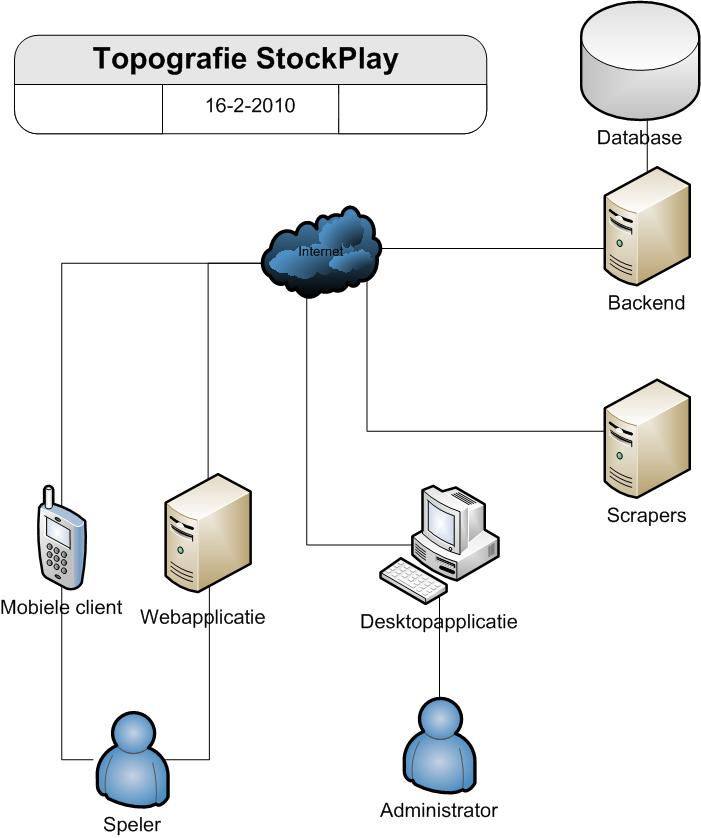
\includegraphics[width=0.5\textwidth]{images/ontwerp/topografie}
	\caption{Topografie van de verschillende systemen.}
\end{figure}

\subparagraph{Scrapers}
StockPlay gebruikt de echte bestaande effecten in het spel. De koersen van deze effecten moeten dus periodiek worden opgehaald om het spel te laten werken. Hiervoor maken we gebruik van in Perl geschreven scrapers die
vanaf enkele vooraf bepaalde sites de koersen extraheren. (vb. \makeurl{De Tijd}{http://www.tijd.be/beurzen/euronext-brussel/continumarkt} of \makeurl{Beursduivel}{http://www.beursduivel.be/koersen-belmid.index}) Hiervoor wordt oa. handig gebruik gemaakt van de AJAX-requests die deze websites gebruiken om de koersen live te tonen. Dit zorgt ervoor dat bijna enkel de koersen worden opgehaald, zonder extra overhead (zoals de layout van de website, etc). Bijkomend voordeel van het gebruik van AJAX is dat Perl libraries voorziet waarmee JSON gemakkelijk ontleed kan worden.
De opgehaalde informatie wordt vervolgens doorgestuurd naar de backend dewelke deze koersinformatie vervolgens opslaat in de database. 

\section{Uitwerking User interfaces}
\subsection{Webapplicatie}

\begin{figure}[h!]
	\centering
		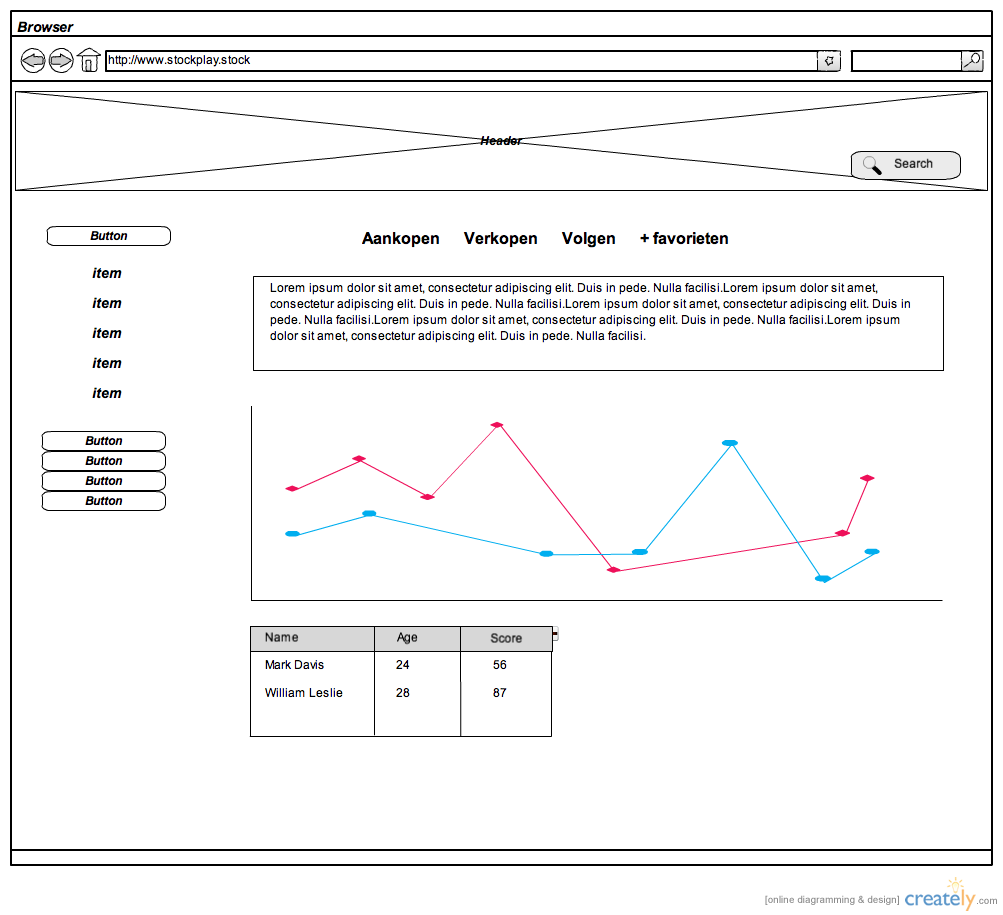
\includegraphics[width=0.5\textwidth]{images/ontwerp/screenshot_website}
	\caption{Layout van de website.}
\end{figure}

Deze interface wordt gebruik om deel te nemen aan het spel. Een gebruiker surft hierbij naar de server die de interface host, en krijgt zo de spelomgeving te zien, dit zonder eerst aan bepaalde softwarevereisten (zoals een Java runtime) te moeten voldaan hebben. Een deel van de functionaliteit is beperkt tot geregistreerde gebruikers, maar meer hierover in hoofdstuk X.

\paragraph{De algemene overzichtspagina}
Deze pagina geeft de gebruiker een zicht over:
\begin{itemize}
	\item{de huidige waarde van de aangekochte effecten en de meer- of minwaarde op de aankoopprijs}
	\item{zijn cashpositie}
	\item{het totaal van zijn cashpositie en de huidige waarde van de effecten}
	\item{het huidige rendement}
	\item{een grafiek met een overzicht van hun rendement ten opzichte van het gemiddeld rendement, beste rendement, enz.}
	\item{het algemeen klassement en eventuele tussenklassementen}
\end{itemize}

\paragraph{Portefolio}
Vervolgens kan de gebruiker zijn portefolio bekijken, en daar volgende informatie uit halen:
\begin{itemize}
	\item{een overzicht van het portefolio van de gebruiker}
	\item{de effecten momenteel in bezit, aankoopprijs (per stuk en in totaal), huidige koers, rendement en winst/verlies op het aandeel}
\end{itemize}

\paragraph{Overzicht beschikbare effecten}
Er is ook een pagina die een zicht biedt op alle effecten aanwezig in het spel.
\subparagraph{Filters} Om het overzicht te behouden voorziet dat overzicht in verschillende filters:
\begin{itemize}
  \setlength{\itemsep}{1pt}
  \setlength{\parskip}{0pt}
  \setlength{\parsep}{0pt}
	\item{per beurs}
	\item{per type (aandeel, tracker, ...)}
	\item{per index}
	\item{per naam}
	\item{aandelen die als favoriet zijn gekenmerkt door de gebruiker}
	\item{per prijs}
	\item{per volume}
\end{itemize}
\subparagraph{Details per effect}Per aandeel kan vervolgens doorgeklikt worden naar een overzichtspagina, die de volgende informatie biedt:
\begin{itemize}
  \setlength{\itemsep}{1pt}
  \setlength{\parskip}{0pt}
  \setlength{\parsep}{0pt}
	\item{grafiek met koers}
	\item{hoog/laag van de dag}
	\item{huidige koers}
	\item{openingskoers}
	\item{verschil}
	\item{omzet}
	\item{mogelijkheid om te kopen/te verkopen}
\end{itemize}

\paragraph{Transactiegeschiedenis}De gebruiker kan ook een overzicht bovenhalen waarop zijn transactiegeschiedenis zichtbaar is. 
\subparagraph{Details per transactie}Ook hier kan men steeds doorklikken naar een detailpagina in kwestie:
\begin{itemize}
  \setlength{\itemsep}{1pt}
  \setlength{\parskip}{0pt}
  \setlength{\parsep}{0pt}
	\item{het tijdstip}
	\item{het effect}
	\item{het type transactie}
	\item{het aantal}
	\item{de kostprijs voor de transactie}
	\item{de winst/verlies door transactie}
	\item{totaal van uw portefeuille}
\end{itemize}
\subparagraph{Filters}Het overzicht kan worden behouden met behulp van volgende filters:
\begin{itemize}
  \setlength{\itemsep}{1pt}
  \setlength{\parskip}{0pt}
  \setlength{\parsep}{0pt}
	\item{enkel aankopen/verkopen}
	\item{enkel met winst/verlies}
\end{itemize}

\paragraph{Klassementen}Er zijn ook verschillende klassementen aanwezig:
\begin{itemize}
  \setlength{\itemsep}{1pt}
  \setlength{\parskip}{0pt}
  \setlength{\parsep}{0pt}
	\item{meest aangekochte aandelen}
	\item{meest verkochte aandelen}
	\item{spelers top 20 (waarde portefolio)}
	\item{spelers top 20 (puntentotaal)}
\end{itemize}

\paragraph{Verhandelpagina effecten}De interface voorziet ook in een pagina om aandelen te kopen of verkopen. Hiervoor zijn verschillende mogelijkheden:
\begin{itemize}
  \setlength{\itemsep}{1pt}
  \setlength{\parskip}{0pt}
  \setlength{\parsep}{0pt}
	\item{de prijs die je biedt voor het aandeel. Pas als het aandeel die koers bereikt wordt het aandeel effectief aangekocht}
	\item{de hoeveelheid aandelen die je wenst aan te kopen}
	\item{de max. geldigheidsduur van dit order (1 uur/dag/week/maand)}
\end{itemize}
Tijdens de aankoop krijgt de gebruiker een overzicht van de totale kostprijs en de verschillende taksen die erop staan.

\subsection{Desktopapplicatie}
Deze applicatie voorziet in het beheer van het hele systeem. De beheerder logt daarvoor in met behulp van zijn eID.
De desktopapplicatie is opgesplitst in drie grote componenten.

\paragraph{Systeemstatus}Het laatste grote deel van de applicatie biedt een overzicht van de systeemstatus. Daarbij kan de beheerder het volgende ondernemen:
\begin{itemize}
\item{status van de componenten (scraper, database, website, ...) en starten/stoppen/herstarten van degene die dit aankunnen.}
\item{statistieken bekijken}
	\begin{itemize}
	\item{aantal ingeschreven gebruikers sinds de start}
	\item{aantal gebruikers online}
	\item{aantal connecties per tijdseenheid op de backend}
	\item{aantal transacties per tijdseenheid}
	\item{aantal (succesvol/gefaalde/...) gescrapede aandelen per tijdseenheid}
	\end{itemize}
\end{itemize}

\begin{figure}[h!]
	\centering
		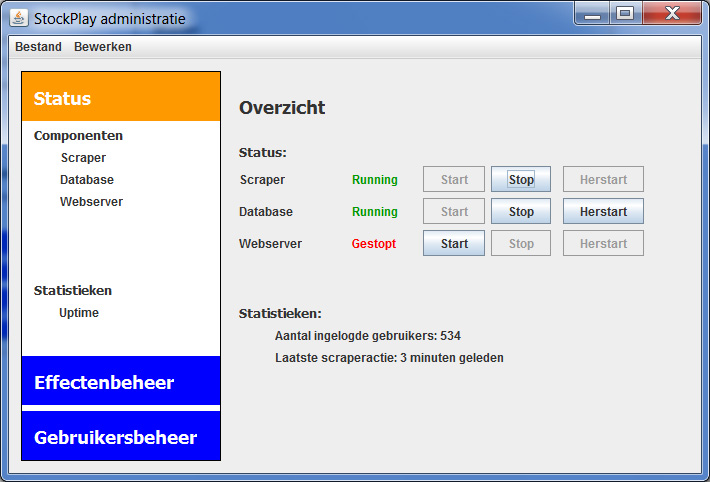
\includegraphics[width=0.5\textwidth]{images/ontwerp/screenshot_app_status}
	\caption{Screenshot van concept statuspagina.}
\end{figure}

\paragraph{Effectenbeheer}Er is ook een overzicht van de effecten voorzien, die de volgende functionaliteit biedt:
\begin{itemize}
	\item{aanduiden van welke effecten moeten gescraped worden, welke effecten zichtbaar zijn bij de spelers}
	\item{schorsen van handel in een effect}
	\item{wijzigen van de gescrapede gegevens}
	\item{overzicht van de aanwezigheid in portefeuilles bij spelers}
\end{itemize}

\begin{figure}[h!]
	\centering
		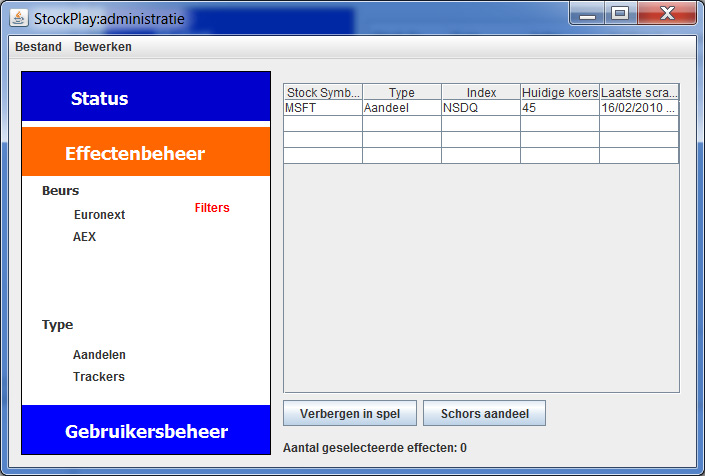
\includegraphics[width=0.5\textwidth]{images/ontwerp/screenshot_app_effecten}
	\caption{Screenshot van concept effectenbeheer.}
\end{figure}

\paragraph{Gebruikersbeheer}Enerzijds is er het overzicht van de gebruikers. Per gebruiker zijn de volgende beheersopdrachten mogelijk: 
\begin{itemize}
	\item{wijzigen van een gebruiker}
	\item{verwijderen van een gebruiker}
	\item{aanpassen van portefolio: kopen/verkopen van effecten}
	\item{de hoeveelheid cash van de gebruiker aanpassen}
\end{itemize}

\begin{figure}[h!]
	\centering
		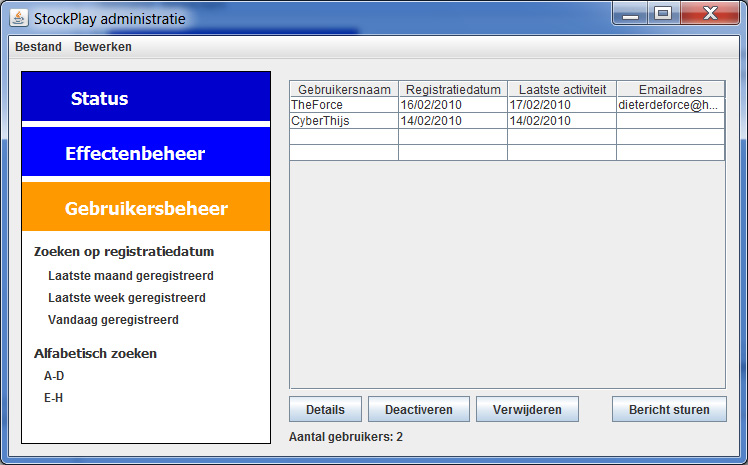
\includegraphics[width=0.5\textwidth]{images/ontwerp/screenshot_app_gebruikers}
	\caption{Screenshot van concept gebruikersbeheer.}
\end{figure}

\section{Backend}
\todo{hoort dit hier?}
Om te vermijden dat alle interfaces gedetailleerde informatie over het databaseontwerp moeten hebben, abstraheren we alle toegang tot de database via een backend. Als een client applicatie dan bepaalde informatie nodig heeft, of wijzigingen wilt toepassen, zal dat gebeuren via een uniforme interface die de backend implementeert. Het exacte ontwerp van deze interface, en de implementatie ervan, kan gevonden worden in een verder hoofdstuk.


%
% Technisch
%

\chapter{Technisch ontwerp}

\section{Hergebruik}

\todo{Beschrijving van het wat en waarom van libraries}

\section{Hardware}

\todo{Een vermelding van de PDA-interface}
